\chapter{Conception}

Le programme développé ici est supposé répondre à un besoin bien précis, c'est-à-dire l'accessibilité d'une ressource bien définie et son utilisation, que ce soit par un utilisateur humain ou par une intelligence artificielle développée spécifiquement pour le jeu souhaité. La première partie de ce projet a donc été dédiée à la conception de ce projet par les besoins d'un utilisateur quel qu'il soit.\\

Ci-dessous sont détaillés les scénarios d'usage du logiciel, ainsi que leurs diagrammes de séquence associés. C'est l'ensemble de ces éléments qui nous a permis par la suite de cerner le cœur de ce qui est attendu à la fin de ce sujet.\\


\begin{figure}[!ht]
	\center
	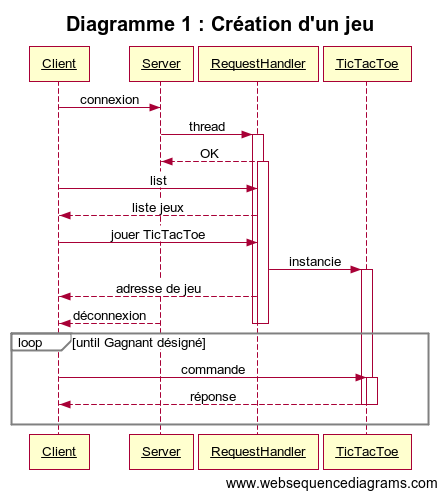
\includegraphics[scale=0.5]{images/sequence/diagramme_scenario1.png}
	\caption{Le premier cas d'utilisation, basique}
\end{figure}